\chapter{Data Preparation}
\label{data_preparation}
%\begin{figure}[H]
%	\centering
%	\begin{tikzpicture}[node distance = 4cm, auto]
%	% Place nodes
%	\node [block] (matrix) {Create similarity matrix for glare effect};
%	\node [block, right of=matrix, node distance=5cm] (mapping) {Mapping};
%	\node [block, right of=mapping, node distance=5cm] (valid) {Valid logs collection};
%	\node [block, below of=matrix] (quality) {quality plotting};
%	\node [block, below of=mapping] (sorting) {Sorting of logs};
%	\node [block, below of=valid] (simulate) {Simulation};
%	\node [decision, below of=quality, node distance=4cm] (decide) {Are simulated logs realistic?};
%	\node [block, below of=simulate] (change) {Change simulator};
%	\node [block, below of=decide] (generate) {Generate features};
%	\node [block, below of=change] (train) {Proceed with traning};
%	
%	% Draw edges
%	\path [line] (matrix) -- (mapping);
%	\path [line] (mapping) -- (valid);
%	\path [line] (valid) -- (simulate);
%	\path [line] (simulate) -- (sorting);
%	\path [line] (quality) -- (decide);
%	\path [line] (sorting) -- (quality);
%	\path [line, pos=0.12] (decide) -- node {No}(change);
%	\path [line] (change) -- (simulate);
%	\path [line] (decide) -- node [midway] {Yes}(generate);
%	\path [line] (generate) -- (train);
%	
%	\end{tikzpicture}
%	\caption[Bild kurz]{hi}
%\end{figure}
To prepare the data for the training many steps were neccesary. One big step is to increse the available dta by simulaing user behaviour. Therefore the simulator	tor in chapter \todo{ref} is used. For simulating games with no opbstacle there is no need for a similarity matrix. However, in order to sucessfully simulate glare effect games, a special similarity matrix is required. While without any obstacles the color differnes are independent from the position of the crads, this is not the case in glare effect games since the intensity of the light is not the same across the whole field. As a result the first step is to create a similarity matrix that descirbes the differneces of colours under the influence of the glare effect. Once completed, it replaces the old similarity matrix in the glare effect logs. As not all logs are valid and can be used in the simulator, the invalid log must be removed. These valid logs are then used to simulate user behaviour and thereby create new logs. These simulated logs are sorted by their quality and the simualtion is evaluateed. If the performance in the simulated games is similar to that in the original games it is preceeded with the gerneration of the features for the training. Otherwise changes to the simulator ar made and the simulation, the sorting and the evaluation are repeated. In case of very bad simulations of glare effcet logs it would have also been possible to change the approch of creating the similarity matrix or find a new approch. However, the simualtinos of glare effect were very good, which can be seen in \todo{ref}, which is why the spproach was kept.

\section{Similarity matrix creation}
\label{similarity_matrix_cretion}

%\section{Glare effect similarity matrix}
%\subsection{Matrix generation}
\subsection{Conceptualization}
\label{conceptualization}
The aim is to create a similarity matrix that descibes the differneces between colours under the influence of the simulated sun light. The difficulty hereby is that the intensity of the light is not spread evenly across the whole field. Instead, as it would be if a real sun would shine onto the display, a certain are has the highest intensity and the intensity is lower the further away from that area. Adittionally there are wide lines of higher intensity comming from the brightest area, that simulate sunbeams. This influence of the simulated sunlight can be seen in figute \ref{fig:glareEffect}. 

\begin{figure}[H]
	\centering
	
\includegraphics[width=14cm]{images/glareEffect.png}
	\caption[Bild kurz]{Screenshot of the game field with simulated sunlight. Sunbeams are especially visible on the right hand side. All cards are turned face up.}
	\label{fig:glareEffect}
\end{figure}
\todo{vielleicht bild raus nehmen weil es oben schon einmal ist und referenzien nach oben}

As a result simply extracting the rgb values for one pixel of each card in one game and calculating the differneces has two major problems: Firstly, the differences are highly influenced by the position of the specific cards. If the matrix is calculated using a single glare effect game the differneces are only representative for exactly that game and may be completely differnet if the cards are positioned differently. Secondly, extracting single pixels for each card in an image could lead to color values that do not represent the overall observed colour due to varying brightnesses on differnet points of a card. This behaviour is undesired, as the final similarity matrix is supposed to represent the differneces of the observed colours of the cards. \todo{vielleicht quelle suchen die sagt das menschen farbenm ion bereichen mitteln oder so} In order to solve these problems a more complex approach then simply extracting single pixels out of a game was needed. 

The problem of the positional influence can be solved by creating similarity matrices for more than one game and calculating the mean color differences of those matrices. The idea is that by creating using so many games that all or most combinations of positions and colours are included and calculating the mean of all comparissons for , the result will not be influenced by the position of the cards.  However, first needs to be determined which number of games satisfies this condition. Each game consists of 14 cards, with each two cards having the same colours. When determining the difference between two colours there are two differnet cases: 
\begin{itemize}
	\item 1. The colours are not the same: In each game there are exactly 4 combinations of positions for those two colours, because there are two cards for each colour. 
	\item 2. The colours are the same: In each game there is only one combination of positions for those colours.  
\end{itemize}

\begin{figure}[H]
	\centering
	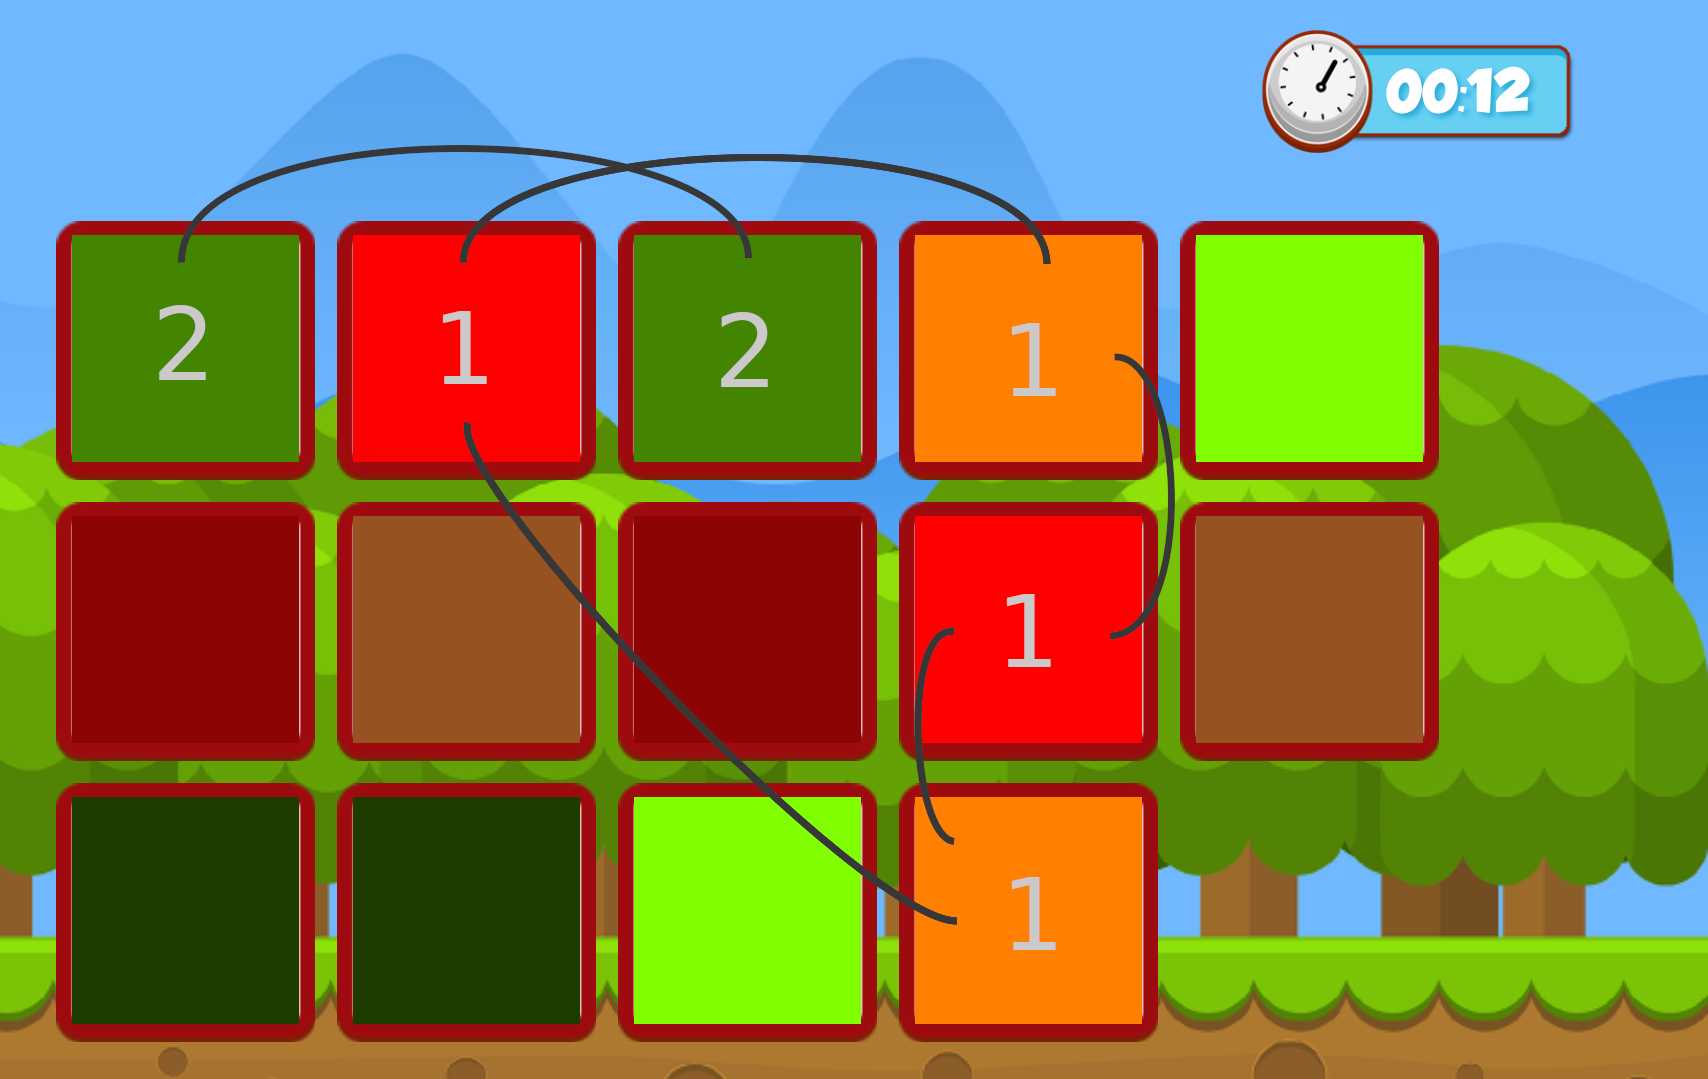
\includegraphics[width=14cm]{images/noObstTurnedNotes.png}
	\caption[Bild kurz]{Examplary showing the number of different comparissons for case 1 and 2. The numbers on the cards represent the case and the edges indicate unique comparissons. All cards are turned face up. A game without any obstacles is used only for the purpose of clarifying the differnet comparissons. All screenshots used for the actual calculation are taken from glare effect games.}
	\label{fig:noObstTurnedNotes}
\end{figure}

First it is calculated how many screenshots are necessary for the first case. For two different coloured arbitrary but fixed cards there can be 
\begin{equation*}
C\textsubscript{1} = 14 \cdot 13 = 182 
\end{equation*}
combinations of positions are possible. The reason that it is not not 14 $\cdot$ 14 is that 14 comparissons of cards with themself would be included. We formulate the condition that enough screenshots need to be taken so that a arbitrary but fixed combination of positions for two different colours is included with a probability of 95\%. 

\begin{center}
	As there are 4 such combinations of positions in each game the probanility P(A) to get a specific combination in a game is 
	\begin{equation*}
	P(A) = \frac{4}{182} % = 0.02198
	\end{equation*}
	The counter probability P($\lnot$A) is 
	\begin{equation*}
	P(\lnot A) = 1 - \frac{4}{182} = \frac{178}{182}%0.02198 = 0.97802
	\end{equation*}
	The number of necceary screenshots to include a specific combination with 95\% probaility is calculated by solving
	\begin{align*}
	1 - P(\lnot A)^n &\geq 0.95 \\
	1 - \left(\frac{178}{182}\right)^n &\geq 0.95 \\
	1 &\geq 0.95 + \left(\frac{178}{182}\right)^n\\
	\left(\frac{178}{182}\right)^n &\leq 0.05\\
	n &\geq log_{(\frac{178}{182})}(0.05) \\
	n &\geq 134.8024 %\llap{$\implies$\hspace{50pt}} at beginnging for implication arrow
	\end{align*}
\end{center}
This means that about 135 Screenshots of games are needed in the first case. Now we perform the same calculation for the second case where there is only one combination of positions for the colours. However, there are less combinations of positions that are relevant than in the first case. For example for two green cards at index 0 and 1 the 182 comparissons would include a comparison of the first green card and the second green card as well as a comparisson of the second green card and the first green card. This goes for every two cards with the same colour, meaning there are only half as many different comparissons in the second case than in the first case. As a result the number of possible combinations in the second case is
\begin{equation*}
C\textsubscript{2} = \frac{C\textsubscript{1}}{2} = \frac{14 \cdot 13}{2} = 91.
\end{equation*}
Now we calculate how many screenshots must be taken to include a specific combination of positions for two equal colours with a probability of 95\%. 
\begin{center}
	As there is one such combinations of positions in each game the probanility P(A) to get a specific combination in a game is 
	\begin{equation*}
	P(A) = \frac{1}{91} % = 0.02198
	\end{equation*}
	The counter probability P($\lnot$A) is 
	\begin{equation*}
	P(\lnot A) = 1 - \frac{1}{91} = \frac{90}{91}.%0.02198 = 0.97802
	\end{equation*}
	The number of necceary screenshots to include a specific combination with 95\% probaility is calculated by solving
	\begin{align*}
	1 - P(\lnot A)^n &\geq 0.95 \\
	1 - \left(\frac{90}{91}\right)^n &\geq 0.95 \\
	1 &\geq 0.95 + \left(\frac{90}{91}\right)^n\\
	\left(\frac{90}{91}\right)^n &\leq 0.05\\
	n &\geq log_{(\frac{90}{91})}(0.05) \\
	n &\geq 271.111 %\llap{$\implies$\hspace{50pt}} at beginnging for implication arrow
	\end{align*}
\end{center}
This means that about 272 screenshots of games are needed in the second case. As there are more screenshots needed for the second case, the first case is also included. This inclusion is caused by the fact that each screenshot includes comparissons for the  fist  as well as the second case. To have a buffer the decision was made to take screenshots of 300 games. In theory these screenshot include any arbitrary but fixed combinations of positions and colours with a probability of over 95\%, which should eliminate the problem of the positional influence.

Nonetheless, this does not solve the second problem of extracting single pixels that can potentially be directly in the area of a sunbeam. This can be fixed, by extracting all pixels in a certain are of the card and averaging their rgb values.  %By averaging all colours in a certain area, the result will be more representitive of what the player actually sees \todo{Quelle finden wo sowas über visuellen kram gesagt wird}. 

Last but not least it needs to be clarified how the colour differneces are calculated. To capture how colour differences are observed by humans, the rgb colour scale is not suitable. Using the rgb colour scale simirlarly stromng perseaved color differnces do not neccessarily have the same eucliidean distance. Contrary to that the CIELAB colour space aims to do exaclty that. Although not perfect, it more accurately descirbes human colour perception than the rgb colour space. Therefore the colour differences described in the similarity matrix are calculated after converting the colours into the CIELAB colour space. The colour distance is called Delta E score. The lower this score is the more similar appear the colours to human eyes. In related work, when creating the similarity matrix for the effect of colour blindness, the CIE1976 colour model was used for the calculations. However, the formula for calculating the colour difference has since then been improved multiple times, resulting in the CIE2000 colour model. Through multiple modifications of the formula it got closer to a visual equidistance, meaning simirlarly stromng perseaved color differnces have more similar Delta E scores than before. Therefore when creating the similarity matrix for the glare effect the CIE2000 colour model is used instead of the old one. 

To sum it up, the chosen approach is to take 300 screenshots of glare effect games with all cards turned face up, extracting areas of rgb values for each card, converting the average rgb values of ares into CIELAB colours, calculating a similarity matrix for each game that contains the delta E scores and finally averaging the delta E scores across all similarity matrices. To achieve values between 0 and 1, the colour differneces additionally need to be scaled down in the end.
 
\subsection{Screenshot extraction}
\label{screenshot_extraction}
To play the memory game and take screenshots an emulator for the pixel 2 in android studio was used. In order to take the screenshots in the needed way and collect additionally necessary information some changes to the memory game were made. In the way the game is intended there are always only maximum two cards turned face up. However, for the screenshots all cards need to be turned around so that the colour differneces can be calculated. Therefore the memory game was adjusted so that all cards are turned face up once the player turns a card. Additionally it was changed so that cards stay face up once they get turned around for the first time. This makes it possible to take screenshots with the colours of all cards visible. Furthermore, for the creation of the similarity matrix it needs to be known what the original colours without the influnece of the simulated sun are. To collect the screenshots and the according colours of the cards in each game a semi-automatic approach was chosen. Once a game is started and a card is flipped, resulting in all cards being turned face up, the colours of all cards are saved in a list. Then a screenshot is manually taken and afterwards the game is exited to enter the main menu. From there on the process is repeated 300 times. As a result there are 300 hundred screenshots of games and a two dimensional list that includes the colours of the cards in the 300 games. The first dimension specifies the game and the second dimension the index of the card. The values of this list are stored in a text file before the game is completely closed. To assure that no mistakes were made when taking the screenshots, the number of collected screenshots is observed during the whole process and afterwards all screenshots are manually checked so that all cards are turned face up.

\subsection{Implementation}
\label{implementation}
This section will show and explain the implementation of the similarity matrix generation. Code is only included if it helps to further understand what is being explained. First of all the screenshots and the information about the original colours of the cards are loaded. Before the actual calculation of a similarity matrix for each image, the average rgb values of the cards on the field need to be determined. 

\begin{lstlisting}[language=python, caption=Add caption, xleftmargin=5.0ex]
def determine_glare_rgb_values(image):
'''
Calculates the rgb average rbg values for each card in an image.
:param image: The screenshot of the memory game with all cards 
turned face up.
:return: The average rbg values in the specified 150 x 150 pixel 
areas for each card. 
'''
glare_rgb_values = []
for corner in card_corners:
	x_border = corner[0] + 150
	y_border = corner[1] + 150
	card_values = []
	for x in range(corner[0], x_border, 1):
		for y in range(corner[1], y_border, 1):
			coordinates = x, y
			pixel_values = image.getpixel(coordinates)
			card_values.append(pixel_values[:-1])
	card_r = int(round(np.mean([color[0] for color in card_values])))
	card_g = int(round(np.mean([color[1] for color in card_values])))
	card_b = int(round(np.mean([color[2] for color in card_values])))
	glare_rgb_values.append((card_r, card_g, card_b))
return glare_rgb_values 
\end{lstlisting}
The cards are each 250 $\cdot$ 250 pixels big and the rgb values are extracted from squared 150 $\cdot$ 150 pixel areas. The coordinates the pixels are extracted from are manually selected in gimp. As a result the areas are only correct for the used resolution of 1080p. Once the mean rgb values in those areas are calculated and converted into LAB colours the similarity matrix can be created. LAB colours are neccessary to calculate the colour differnece using the CIE2000 colour model. Each of the 28 cells in the similarity matrix falls into one of the two cases explained in \todo{ref}, meaning there are either 4 or only 1 unique combination for the calculation of each cell value. For every combination the lab colour distance is determined and the values for each cell are averaged. This completes the steps for a single image, resulting in a similarity matrix with unscaled values. 
%\begin{lstlisting}[language=python, caption=Add caption]
%def determine_distance(color_1_rgb, color_2_rgb):
%	'''
%	Determines dinstance between colors with delta e formula. 
%	:param color_1_rgb: The first color.
%	:param color_2_rgb: The second color.
%	:return: The delta_e distance between the two colours. 
%	'''
%	lab_1 = convert_color(color_1_rgb, LabColor)
%	lab_2 = convert_color(color_2_rgb, LabColor)
%	
%	if cie_1976:
%		detlta_e = delta_e_cie1976(lab_1, lab_2)
%	else:
%		detlta_e = delta_e_cie2000(lab_1, lab_2, Kl=1, Kc=1, Kh=1)
%	return detlta_e
%\end{lstlisting}
Once a similarity matrix with unscaled values for every image is created, the average of all matrices is calculated. During the whole calculation of the single matrices it is being kept track of the highest occurring colour differnece. The last step neccessary to complete the final similarity matrix is to divide all values in the matrix by use the highest colour differnce to scale them down to be between 0 and 1. 

%Through the original colours loaded in the beginning, the coverage of combinations in the 300 games can be calculated. 
%\begin{lstlisting}[language=python, caption=Add caption]
%def determine_coverage(original_colors):
%'''
%For calculating how many of the combinations are includes 
%in the calcuation. 
%The calculations are based on having 14 cards on the field.
%:param original_colors: A list containing tuples with the card name, 
%the mappimg number for the card, and the index for each card on the 
%screenshot for all screenshots.
%:return: The coverage of combinations of positions 
%for all colour combinations. 
%'''|\Suppressnumber|

%[...]|\Reactivatenumber{18}|

%combinations = []
%for colors in original_colors:
%for i in range(len(colors)):
%original_color_1 = colors[i]
%for l in range(len(colors)):
%original_color_2 = colors[l]
%if original_color_1[2] != original_color_2[2] and (original_color_2, original_color_1) %not in combinations and (original_color_1, original_color_2) not in combinations:
%combinations.append((original_color_1, original_color_2))    
%return len(combinations) / number_of_total_combinations
%\end{lstlisting}

\subsection{Testing}
\label{testing}
To verify the correcteness of the color extraction and the calculation of the similarity matrix, the main funtionalities are manually tested. The colour extraction was tested by extracting colours of a screenshot with the skript and compoaring the rgb values to the actual values in the images using gimp. Furthermore the calculation of the delta e score was tested, by comaring results of the script with those of an online calculator. \\

To assure that the 300 games actually include most of the combinations and therefore eliminate the positional influence of cards, the coverage of combinations can be additionally calculated. Therefore the number of unique combinations included in the 300 screenshots must be divided by the overall number of possible combinations. The number of unique combinations can be counted during the process of creating the similarity matrix, but the number of possible combinations must seperatly be determined. The similarity matrix for glare effect has 28 entries, from which 7 are comparissons between same and 21 between different colours. With \textit{C\textsubscript{1}} and \textit{C\textsubscript{2}}  being the possible combinations for two arbitrayry but fixed coloured cards in the two cases mentioned above, the number of overall possible combinations C is
\begin{align*}
	C &= 21 \cdot C\textsubscript{1} + 7 \cdot C\textsubscript{2}\\
	&= 21 \cdot 182 + 7 \cdot 91\\
	&= 4459. 
\end{align*}
The 300 games used for creating this matrix include 99.57\% of all possible combinations. Furthermore is was verified that certain combinations are not included significantly more often than others and in that sense have stronger influence on the result. \todo{code ergänzen und nachprüfen wie oft die combinationen vorkamen..histogramm?}. 

\subsection{Final Matrix}
\label{final_matrix}
In figure \ref{fig:simMatrix} the final similarity matrix can be seen, dsiplaying how colour differneces are observed under the influence of the simulated sunlight, averaged over 300 games. As mentioned before, the lower the delta e score the more similar the cards appear to the human eye. The maximum delta E score that occured during the calculation was 8.861. All values are divided by that number to achieve scores between 0 and 1.
%maximum distance: 8.861003756554735.
\begin{figure}[H]
	\centering
	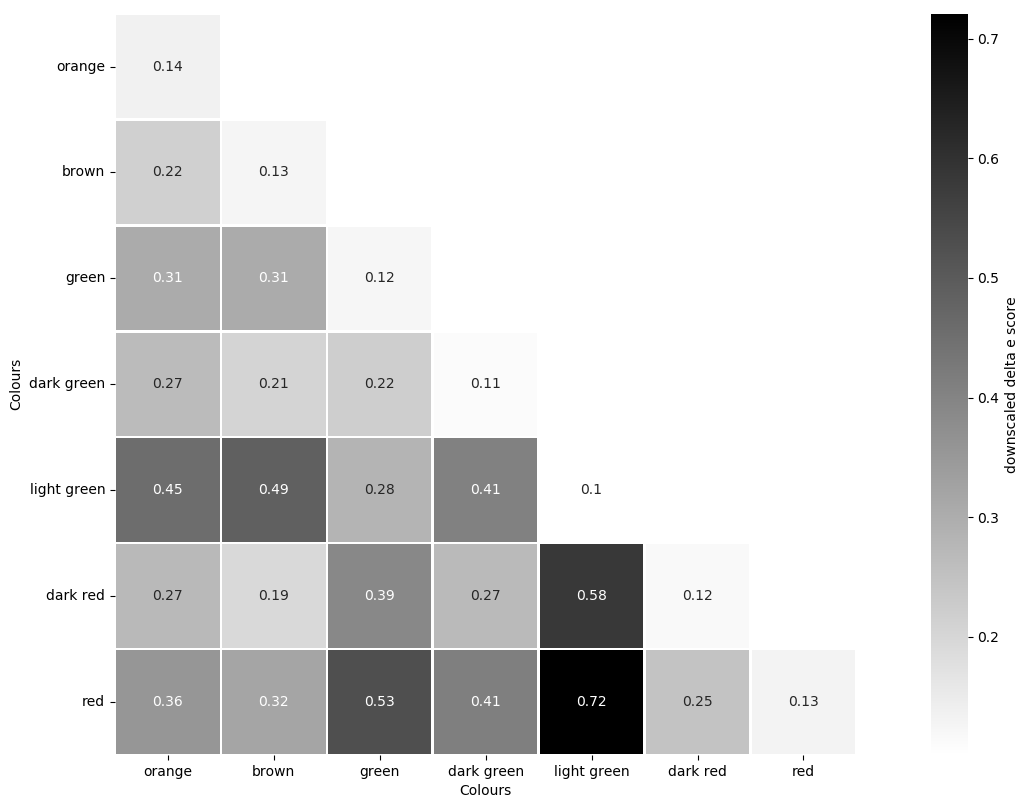
\includegraphics[width=15cm]{images/simMatrixGrey.png}
	\caption[Bild kurz]{Add caption. The lighter the colour the less a difference is noticeable}
	\label{fig:simMatrix}
\end{figure}
The delta E score is less a definitive answer, and instead a helpflu metric to apply to a specific use case. Although there are tendencies regarding the interpretation of colour differences, there is no definitive table that descriebes what the different scores mean. One reason for this is that the perceived colour differnece may vary in different situations and circumstances. For instance, is the colour difference perceived differently depending on how long the colours are exposed to the human eye, as humans can over time adapt to the colours. This means that in a setup where all colours are always visible the colour difference will likely be perceived weaker than in the case of the memory game, as the cards are only flipped momentarily, leaving little time for adaptation. Table ref was created through own observation and in that sense is highly influenced by the strength of the sense of sight from the creator of this work. Therefore it should not be taken definitive but only serve the purpose of claryfying how the values in the matrix can roughly be interpreted.
\begin{table}[H]
	\centering
	\caption{add caption.}%\label{tab1}
	\begin{tabular}{|c|c|c|}
		\hline
		Delta E & Downscaled values & Perception of difference \\
		\hline
		$\leq1.33$ & $\leq0.15$ & Not perceptible by human eyes\\
		$1.33-2.66$ &$0.15-0.3$  & Only perceptible through close observation \\
		$2.66-4.43$ & $0.3-0.5$ & Perceptible colour difference \\
		$\geq4.43$ &$\geq0.5$  & Major colour difference\\
		\hline
	\end{tabular}
\end{table}
Before actually using the constructed simialry matrix in the simulator it is unknown if the chosen approach results in high quality simulations. If this is not the case it is possible to change the concept or try other approches. 

It should be also noted that the similarity matrix has 28 entries. The one that was used for describing the confusion that happens during colour blindness only has 21 entries, because all 7 values describing cards of the same colour can be left out as the colours are equal. Since in glare effect games, originally equally coloured cards can look due to the influence of the simulated sunlight, these 7 values must be included in the similarity matrix for the glare effect.

\section{Incorporation of the new similarity matrix}
\label{incorporation_of_the_new_similarity_matrix}
The former similarity matrix in the glare effect logs that was just a placeholder can now be replaced with the newly created one. To do so there was already a script available, that was used after some small adjustments. The main changes were to replace the deprecated functions from libraries with supported ones and incorporate the new similarity matrix. As the code was initially written for similarityg matrices with 21 entries and the one for glare effcet has 28 entries, the code for that created the dynamic similarity assignments the logs had to be adapted. Finally all remapped logs are saved in new files. To check whether the remapping is still done correctly, the resulting logs were compared to logs that were remapped by the original script. The only thing that was not original were the replaced deprecated functions as this was neccesary to execute the script. Besides differnet similarity values due to differnet matrices as well as the fact that the logs now also contained entries for same coloured cards, the mapping was identical. 

%One problem with the logs is, that the mapping was done statically when they were created. However, the simulator requires dynamic mapping. The difference is emplained in chapter \todo{ref}. To do so there was already a script available, that was used after replacing some deprecated functions from libraries with supported ones. Furthermore the code was extended so that the old placehoulder similarity matrices in the logs are replaced by the new one. As the code was initially written for similarityg matrices with 21 entries and the one for glare effcet has 28 entries, the code for remmaping the logs had to be adapted. Finally all remapped logs are saved in new files. To check whether the remapping is still done correctly, the resulting logs were compared to logs that were remapped by the original script. The only thing that was not original were the replaced deprecated functions as this was neccesary to execute the script. Besides differnet similarity values due to differnet matrices as well as the fact that the logs now also contained entries for same coloured cards, the mapping was identical. 

\section{Removal of invalid logs}
\label{removal_of_invalid_logs}
For the simualation to work, the game log that is used for the simulation must have had all cards turned around at least once. If this is not the case the log is classified as invalid. Additionally to removing invalid logs, the aim is to create a balanced data set for training. Therefore the number of games in each game mode has to be equal. Using twice as many no obstacle games for training than glare effect games can lead to games being more often classified to have no obstacle only because they appeared more often during training. As a result the model would be less capable of detecting actual visual interaction obstacles. Furthermore the decision was made that the number of games from each participant in each game mode should be equal, too. This means that the data should not contain more no obstacle games from a particiapnt than glare effect games, and vice versa.
%\todo{consicder precision and recall in real world scenarios? but can i assume anythn? For instance that people are less often blinded than no}.  

As stated in chapter \todo{ref} from the 22 participants there are 44 no obstacle and 21 glare effect game logs. To collect the data used for the simulation, a script was written that collects one no obstacle and one glare effect log from each participant. Half of the available no obstacle logs are not collected, because there are not as many glare effect logs. Once the logs are collected, they are validated and the valid ones are saved in new files. If at least one the two logs from a participant from different game modes is invalid, both are removed. Otherwise the training data would be inconsistent in that sense that the logs from different game modes could be from different participants. From the 22 no obstacle and 21 glare effect logs collected by the script, one glare effect log was invalid. This resulted in 20 no obstacle and 20 glare effect logs being used for simulation. These 40 real logs combined with those simulated form the data used for training. 
\begin{lstlisting}[language=python, caption=Add caption, xleftmargin=5.0ex]
def validate_log(log):
	'''
	Validates logs.
	:param log: The log to validate. 
	:return: If the log is valid.
	'''
	needed_entries = ['1.1,', '2.1,', '3.1,', '4.1,', '5.1,', '6.1,', '7.1,', '1.2,', '2.2,', '3.2,', '4.2,', '5.2,', '6.2,', '7.2,']
	for needed_entry in needed_entries:
		if needed_entry not in log:
			return False
	return True
\end{lstlisting}

\section{Simulation of user behaviour}
\label{simulatoin_of_user_behaviour}
The whole process of simulating user behaviour is divided into two parts: First configuartion files are created, using a generic optimization algorithm, that contain the optimized parameter values and secondly these configuration files are used to simulate games. How the simulator functions is explained in chapter \todo{ref}.

Multiple additions were made to the simulator. In total four classes were added. Two are for generating configuration files for the simulation of game with and without the glare effect obstacle %(NoObst\_ConfigGenerator\_dataCollection2020.java and GlareEffect\_ConfigGenerator\_dataCollection2020.java) 
and the other two for using those files to simulate new games based on the user behaviour in the original games.  %(NoObstWinStrategyTrainingDataGenerator\_dataCollection2020.java and GlareEffectWinStrategyTrainingDataGenerator\_dataCollection2020.java)
These classes utilize the functionalities already implemented in the simulator. However, as the simulator only worked with similarity matrices that have 21 entries, instead of the 28 of the matrix for glare effect games, the simulator was adjusted so that it can also handle matrices with 28 entries. After all changes and additions were completed, each log was used to simulate 1000 games, resulting in 40000 logs. From these logs 20000 are no obstacle games and the other 20000 are glare effect games. The 40000 logs contain 1000 no obstcle and 1000 glare effect logs for each of the 20 probants.  

%Multiple additions were made to the simulator. In total four classes were added. Two are for generating configuration files for the simulation of game with and without the glare effect obstacle (NoObst\_ConfigGenerator\_dataCollection2020.java and GlareEffect\_ConfigGenerator\_dataCollection2020.java) and the other two for using those files to simulate new games based on the user behaviour in the original games (NoObstWinStrategyTrainingDataGenerator\_dataCollection2020.java and GlareEffectWinStrategyTrainingDataGenerator\_dataCollection2020.java). These classes utilize the functionalities already implemented in the simulator. \todo{grob erklären wie code funktioniert? momentan glaube ich eher nicht} However, as the simulator only worked with similarity matrices that have 21 entries, instead of the 28 of the matrix for glare effect games, the simulator was adjusted so that it can also handle matrices with 28 entries. After all changes and additions were completed, each log was used to simulate 1000 games, resulting in 40000 logs. From these logs 20000 are no obstacle games and the other 20000 are glare effect games. The 40000 logs contain 1000 no obstcle and 1000 glare effect logs for each of the 20 probants.  


\section{Sorting logs by quality}
\label{sorting_logs_by_quality}
The siulated logs ware sorted by how close their performance is to that in the real game used for their simulation. The value by which is sorted, is the average of two values. The first one is the root mean squared error (rmse) between the matching pairs in the real and the simulated game for each round. The second one is the rmse between the penalties in the real and the simulated game for each round. These two performance measurements are explained in section \todo{ref}. The formula for calculating the rmse is shown below. 

\begin{equation*}
rmse = \sqrt{(\frac{1}{n})\sum_{i=1}^{n}(y_{i} - x_{i})^{2}}
\end{equation*}

Averaging the two rmse's for each simulated game and sorting the logs accordingly,   makes it possible to only use acertain number of the best simulated logs during the training instead of using all of them or a random subset. 
%For each simulated log the rmse is determined by calculating the distance between the penalties in simulated and real games as well as between the matching pairs in real and simulated games for each round, . per round \todo{klären genau was da gemacht wird mit mazen, ich galube rmse für alle perfomace werte in einem game und dem originalen game} as measurement. This is important because it enables to only use the best n simulated logs for training instead of using all of them or a random subset. 

\section{Evaluation of simulation new}
To evaluate whether the performance in the simlated logs is similar to the one in the original logs two perofmance measurements are used: The matching pairs in each round and the penalties in each round. Penalties are given if a card is revealed whose partner has already been seen before but the pair was not picked up. Some initial observations inspired changes to the simulator. The quality of the simulations regarding the performnce measurements is analysed before and after the changes to the simulator, by comparing the performance between simulations and real games. Furthermore a subset of the simulated data was discovered that mostly shows no significant differnece between the perfromnce of the simulated and the real games.

\subsection{Results before and after changing the simulator}
The Initial simulation results can be seen in figure \ref{fig:simIn1} and \ref{fig:simIn2}. The horizontal line extending from the curves, also calles whiskers, describe the standard deviation of the corresponding value. 

\begin{minipage}{0.5\textwidth}
	\begin{figure}[H]
		\centering
		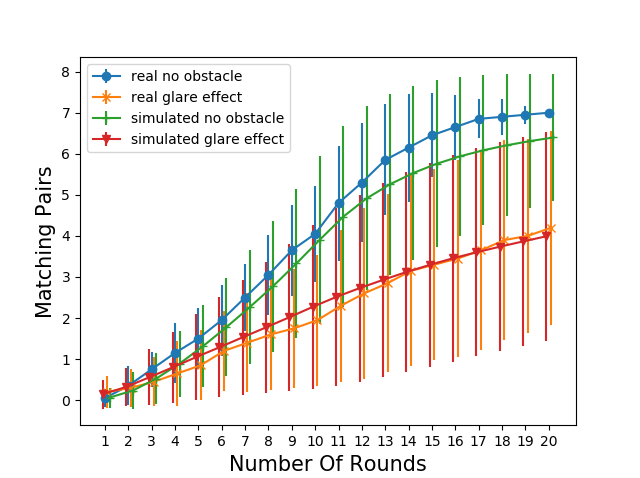
\includegraphics[width=8cm]{images/simulationInitial1.png}
		\caption[Bild kurz]{Add caption}
		\label{fig:simIn1}
	\end{figure}
\end{minipage}
\begin{minipage}{0.5\textwidth}
	\begin{figure}[H]
		\centering
		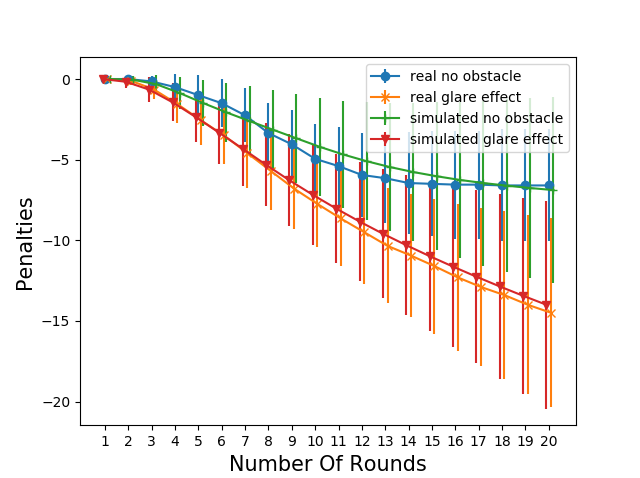
\includegraphics[width=8cm]{images/simulationInitial2.png}
		\caption[Bild kurz]{Add caption}
		\label{fig:simIn2}
	\end{figure}
\end{minipage}

At first glance it can be seen that the simualtions of glare effect games are very similar to the real games, meaning that the constructed similarity matrix creates good simulation results. As a result there is no need to find a different approach for creating the similarity matrix, and no changes to the simulator regarding the simulations of glare effect games are made. However, the simulation of no obstacle games is not quite as accurate. Especially the number of matching pairs after the tenth round in the simulated games is lower than in the real games. Additionally the standard deviation indicated by the whiskers regarding the no obstacle games is noticeably higher in simulated than in the real games. This is not very string in the first turns but gets worse in later turns. Furthermore, however less noticeable, is are the penalties in the simulated games between round 8 and 18 lower than in the real games.

The fact that matching pairs per round for the no obstacle simulations are noticeably lower than in the real games inspired two changes to the simulator. The first one was to introduce a new parameter for the optimization algothithm to optimize. It was called randomizing decy and is a value between 0 and 1, and adresses the problem of worser performance in the löast turn compared to real games. The \textsc{boundary limit}, describing \todo{herausfinden was das ist und erklärung hinzufügen und zuende schrieben}, is multiplied with the randomizing decay each round beginning with the 10th round. This reduces the .. and therefore results in better perfomance in the last 10 steps. The second change was to reduce the probability of revealing a random card (instead of puruing a win strategy) by 0.2 (randomrevealprobabilty is a random value betwen 0 and 1). This was done to increase the overall performance in the simulations by reducing the randomness. The results of these changes can be seen in figure \ref{fig:simOp1} and \ref{fig:simOp2}. 

\begin{minipage}{0.5\textwidth}
	\begin{figure}[H]
		\centering
		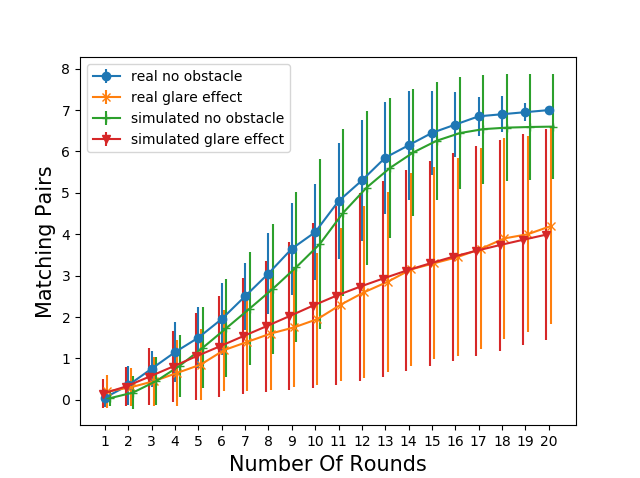
\includegraphics[width=8cm]{images/simulationOptimized1.png}
		\caption[Bild kurz]{Add caption}
		\label{fig:simOp1}
	\end{figure}
\end{minipage}
\begin{minipage}{0.5\textwidth}
	\begin{figure}[H]
		\centering
		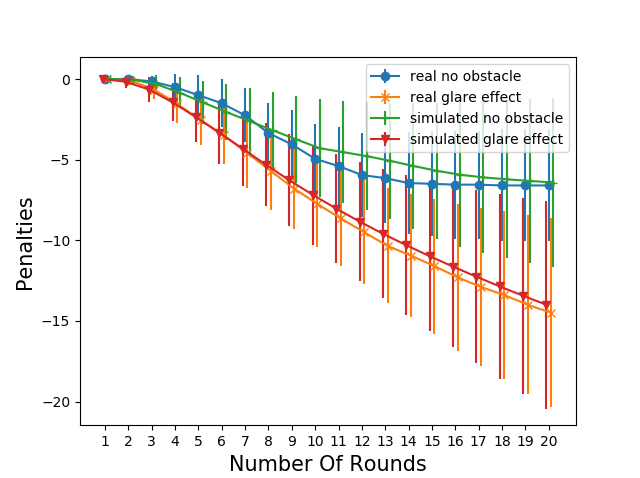
\includegraphics[width=8cm]{images/simulationOptimized2.png}
		\caption[Bild kurz]{Add caption}
		\label{fig:simOp2}
	\end{figure}
\end{minipage} 

As the changes only affected the simulation of no obstacle games, the following statements only refer to those games. It is noticeable that the number of matching pairs per round in the simulated games is closer to the real games. Additionally the standard deviation of the simulated games regarding the matching pairs per round gets noticeably smaller after the 10th round and by that is closer to that in the real games. However, the reduction of randomness also resulted in slightly less penalties after round 10 and by that the differnece in penalties between the simulations and the real games becomes bigger. On the contracry, the standard deviation of the penalties in the last 6 rounds of the simulated no obstacle games got slightliy closer to that in the real games. It seems that the improvements regarding the matching pairs overweight the deteriorations of the penalties, but if these changes actually improve the overall quality of the simulations can not be said without further analysis. 
%will be seen when comparing the classification results before and after the changes. This is done in chapter \todo{ref}. \todo{eigentlich ist das nicht wirklich indiz, vielelict besser: wir untersuchen vorher und nacher mit statistischen test und eventuell auch indication wenn sich die test accuracies unterscheiden später}

However, another interesting observation can be made. The standard deviations of the two perfromance measurements in the last rounds of the simulated no obstacle games is notably higher than in the real games. This might be caused by the fact that there are in generel less or even no cards on the field if all pairs were discovered. This theory also fits to the fact that this is not an issue in the glare effect games, as there are more cards on the field in later turns. This concludes, that there is a possibility that the simulator struggles to accurately simulate rounds once there only a few or no cards remain on the field. 

Although major tendencies of similarities and differences are visually noticable in figure \todo{ref} and figure \todo{ref}, a more accurate analysis is needed to to make reliable statements. Therefore multiple paired samples t-test are performed, comparing real no obstacle, simulated no obstacel, real glare effect and simualted glare effect games with each other. For each combination two tests are performed. One comparing the mean penalties per round and the other one comparing the mean numbers of matching pairs per round. The resulting p values can bee seen in table \todo{ref} and table \todo{ref}. These values express whether the compared lists of mean values are significantly different or not. Values higher than 0.05 indicate no significant difference, while values below 0.05 indicate a significant difference. It would be optimal if all comparissons between different game mode show significant difference, while comparissons between real and simulted games of the same type show no significant difference. All paired sample t-tests were performed before and after the changes to the simulator. This was done to see whether the changes to the simulator improved or deteriorated the results of the test or if they had any impact on them at all. First the results of the paired sample t-tests, when including all 20 rounds and all simulated games, are analysed. Tables \todo{ref} and \todo{ref} show the resuts before changing the simulator, while table \todo{ref} and \todo{ref} show the results afterwards.
%\todo{fertig schreiebn}\\
%It is visble that a improvement to the simulator was made regarding the perfomrance measurements. (ich glaube lkeine statistischen tests fdafür nur wenn ich nopch zeit habe..). Although the graphs show that the simuletad data is very close to the original one, statistcal test will give futher knowledge and certainty. \\
%- t-stochastic test kram (siehe mazens nachricht) -> paired t test: gucken ob no obstacle und glare effet signifikant unterscheidlich sind -> ja sind sie \\
%- vielleicth auch gucken ob verbesserung das signifikant besser gemacht hat, aber kann eventuell auch vernachlässigt werden weil man es visuell sieht und der unterscheid nicht starks sein wird. Dennoch könnte es gut sein dass zu machen. \\
%- auch schriewben was paired ttest überhapt ist und wozu es gut ist.


\begin{table}[H]
	\centering
	\caption{Before change to simulator. p and t values in paired t-test for different comparissons of matching pairs per round. All 1000 simulated games per real game were used. The following abreviatrions are used: real glare effect - r\_g, real no obstacle - r\_n, simulated glare effect - s\_g, simulated no obstacle - s\_n}
	\resizebox{\columnwidth}{!}{%
		\begin{tabular}{|c||ccccc|ccccc|ccccc|}
			
			\hline
			&&& s\_n &&&&& s\_g &&&&& r\_n  && \\
			\hline
			&& p && t &&& p && t &&& p && t & \\
			\hline\hline
			r\_g &&  $1.7e-06$  && $ -6.8179$ &&&  \textcolor{mygreen}{$0.0688$} && $-1.9292$ &&& $9.3e-07$ && $7.1041$ &\\
			r\_n &&   \textcolor{red}{$5.7e-07$}  && $7.3571$ &&& $2.7e-06$ && $6.5765$ &&&     &&     &\\
			s\_g &&  $5.3e-06$  && $6.2480$ &&&  	 &&     &&&     &&     &\\
			\hline
		\end{tabular}
	}
\end{table}




\begin{table}[H]
	\centering
	\caption{Before change to simulator. p ant t values in paired t-test for different comparissons of penalties per round. All 1000 simulated games per real game were used. The following abreviatrions are used: real glare effect - r\_g, real no obstacle - r\_n, simulated glare effect - s\_g, simulated no obstacle - s\_n}
	\resizebox{\columnwidth}{!}{%
		\begin{tabular}{|c||ccccc|ccccc|ccccc|}
			\hline
			&&& s\_n &&&&& s\_g &&&&& r\_n  && \\
			\hline
			&& p && t &&& p && t &&& p && t & \\
			\hline\hline
			r\_g &&  $3.6e-06$  && $-6.4297$ &&&  \textcolor{red}{$1.1e-06$} && $-7.0423$ &&& $3.2e-06$ && $6.4897$ &\\
			r\_n &&   \textcolor{mygreen}{$0.2011$}  && $-1.3242$ &&& $5.6e-06$ && $6.2238$ &&&     &&     &\\
			s\_g &&  $5.4e-06$  && $6.2394$ &&&  	 &&     &&&     &&     &\\
			\hline
		\end{tabular}
	}
\end{table}

\begin{table}[H]
	\centering
	\caption{p and t values in paired t-test for different comparissons of matching pairs per round. All 1000 simulated games per real game were used. The following abreviatrions are used: real glare effect - r\_g, real no obstacle - r\_n, simulated glare effect - s\_g, simulated no obstacle - s\_n}
	\resizebox{\columnwidth}{!}{%
		\begin{tabular}{|c||ccccc|ccccc|ccccc|}
			\hline
			&&& s\_n &&&&& s\_g &&&&& r\_n  && \\
			\hline
			&& p && t &&& p && t &&& p && t & \\
			\hline\hline
			r\_g &&  $5.7e-06$  && $-6.2181$ &&& \textcolor{mygreen}{$0.0688$} && $-1.9292$ &&& $9.3e-07$ && $7.1041$ &\\
			r\_n &&  \textcolor{red}{$1.8e-10$}  && $12.2469$ &&& $2.7e-06$ && $6.5765$ &&&     &&     &\\
			s\_g &&  $1.7e-05$  && $5.7107$ &&&  	 &&     &&&     &&     &\\
			\hline
		\end{tabular}
	}
\end{table}




\begin{table}[H]
	\centering
	\caption{p ant t values in paired t-test for different comparissons of penalties per round. All 1000 simulated games per real game were used. The following abreviatrions are used: real glare effect - r\_g, real no obstacle - r\_n, simulated glare effect - s\_g, simulated no obstacle - s\_n}
	\resizebox{\columnwidth}{!}{%
		\begin{tabular}{|c||ccccc|ccccc|ccccc|}
			\hline
			&&& s\_n &&&&& s\_g &&&&& r\_n  && \\
			\hline
			&& p && t &&& p && t &&& p && t & \\
			\hline\hline
			r\_g &&  $4.8e-06$  && $-6.2967$ &&& \textcolor{red}{$1.1e-06$} && $-7.0423$ &&& $3.2e-06 $ && $6.4897 $ &\\
			r\_n &&  \textcolor{red}{$0.0195$}  && $-2.5519 $ &&& $5.6e-06$ && $6.2238$ &&&     &&     &\\
			s\_g &&  $7.2e-06$  && $6.1045$ &&&  	 &&     &&&     &&     &\\
			\hline
		\end{tabular}
	}
\end{table}


\begin{comment}
\begin{table}[H]
\centering
\caption{p and t values in paired t-test for different comparissons of matching pairs per round. All 1000 simulated games per real game were used. The following abreviatrions are used: real glare effect - r\_g, real no obstacle - r\_n, simulated glare effect - s\_g, simulated no obstacle - s\_n}%\label{tab1}
\begin{tabular}{|c|c|c|c|}
\hline
& s\_n  	&  s\_g  & r\_n 		\\
\hline
r\_g 	&$p=5.7e-06$ &\textcolor{mygreen}{$0.0688$}&$9.3e-07$			\\
r\_n 	&\textcolor{red}{$1.8e-10$}&$2.7e-06$&		  			\\
s\_g 	&$1.7e-05$&			&		  			\\
\hline
\end{tabular}
\end{table}

\begin{table}[H]
\centering
\caption{p values in paired t-test for different comparissons of penalties per round. All 1000 simulated games per real game were used. The following abreviatrions are used: real glare effect - r\_g, real no obstacle - r\_n, simulated glare effect - s\_g, simulated no obstacle - s\_n}%\label{tab1}
\begin{tabular}{|c|c|c|c|}
\hline
& s\_n  	&  s\_g  & r\_n 		\\
\hline
r\_g 	&$4.8e-06$&\textcolor{red}{$1.1e-06$}&$3.2e-06$			\\
r\_n 	&\textcolor{red}{$0.0195$}&$5.6e-06$&		  			\\
s\_g 	&$7.2e-06$&			&		  			\\
\hline
\end{tabular}
\end{table}
\end{comment}

It can be seen that all tests comparing different game mods show significant difference in penalties per round as well as matching pairs per round, which is desired. However significant difference is not dersired in the four test comparing real and simulated games of the same mode, which are highlighted by colours. Before the changes to the simulator, the matching pairs per round in simulated and real no obstacle games show significant differneces. The same goes for the penalties per round in simulated and real glare effect games. As the changes to the simulator only affected the simulation of no obstacle games the significant difference between the matchiung pairs in simulated and real glare effect games prevales. Despite the fact that the matching pairs per round in simulated no obstacle games seem closer to the real games in table figure \todo{ref}, the statistical tests still show a significant differnece between them. Additionally, the small deterioration of the penalties that were caused by the changes to the simulator and can be observed in figure \todo{ref}, led to a significant difference in the penalties per round between simulated and real no obstacle games. Before the changes to the simulator this difference was not significant.  

In total, before the changes to the simulator 2 out of 4 tests comparing games of the same mode, result in undesired significant differences. After the changes to the simulator this increased to 3 out of 4 tests. However, this does not lead to the conclusion that the changes to the simulator decreased the quality of the simulations, as the matching pairs per round in simulated no obstacle game got noticeably more accurate. 

\subsection{Search for a better subset of the data}
In the statictical tests in section \todo{ref}, all all 1000 simulations per participant are used. As some simulations are better than others, using a subset only containing a number of best simulations could lead to further findings. Since the simulated games are sorted by their quality in section \todo{ref}, it is possible to only use a certain number of best simulations for the comparissons, and see whether this improves the undesired properties mentioned above. Furthermore the number of rounds in the comparisson can be changed, so that not all 20 rounds are included. The concideration of including less rounds is of importance, beacuse it can reveal which parts of the game are simulated accurately and which are not. The search for an configuration of those two settings was manually done by varying the number of steps and the ratio between simulated and real data. A configuration of those two settings that produces interesting results consisted of using only the best 10 simulated games per game mode from each participant and only including the first 10 rounds of each game. The results before the changes to the simulator can be seen in table \todo{ref} and \todo{ref}, while the results afterwards are shown in table \todo{ref} and \todo{ref}. The two performance measurements after the changes to the simulator when only using the best 10 simulated games per game mode from each participant are aditionally portrayed in figure \todo{ref} and \todo{ref}.

\begin{table}[H]
	\centering
	\caption{Before change to simulator. p and t values in paired t-test for different comparissons of matching pairs per round. For the simualted data only the best 10 simulated logs from each real log are used. Only the first 10 rounds are used. The following abreviatrions are used: real glare effect - r\_g, real no obstacle - r\_n, simulated glare effect - s\_g, simulated no obstacle - s\_n}
	\resizebox{\columnwidth}{!}{%
		\begin{tabular}{|c||ccccc|ccccc|ccccc|}
			\hline
			&&& s\_n &&&&& s\_g &&&&& r\_n  && \\
			\hline
			&& p && t &&& p && t &&& p && t & \\
			\hline\hline
			r\_g &&  $0.0080$  && $-3.3879$ &&& \textcolor{red}{$6.3e-05$} && $7.0000$ &&&  $0.0058$ && $3.5985$ &\\
			r\_n &&   \textcolor{red}{$0.0047$}  && $3.7292$ &&& $0.0038$ && $3.8679$ &&&     &&     &\\
			s\_g &&  $0.0052$  && $3.6587$ &&&  	 &&     &&&     &&     &\\
			\hline
		\end{tabular}
	}
\end{table}

\begin{table}[H]
	\centering
	\caption{Before change to simulator. p values in paired t-test for different comparissons of penalties per round. For the simualted data only the best 10 simulated logs from each real log are used. Only the first 10 rounds are used. The following abreviatrions are used: real glare effect - r\_g, real no obstacle - r\_n, simulated glare effect - s\_g, simulated no obstacle - s\_n}
	\resizebox{\columnwidth}{!}{%
		\begin{tabular}{|c||ccccc|ccccc|ccccc|}
			\hline
			&&& s\_n &&&&& s\_g &&&&& r\_n  && \\
			\hline
			&& p && t &&& p && t &&& p && t & \\
			\hline\hline
			r\_g &&  $0.0024$  && $-4.1873$ &&& \textcolor{red}{$0.0491$} && $2.2730$ &&&  $0.0014$ && $4.5577$ &\\
			r\_n &&  \textcolor{mygreen}{$0.9426$}  && $0.0740$ &&& $0.0012$ && $4.6629$ &&&     &&     &\\
			s\_g &&  $0.0020$  && $4.2932$ &&&  	 &&     &&&     &&     &\\
			\hline
		\end{tabular}
	}
\end{table}

\begin{table}[H]
	\centering
	\caption{p and t values in paired t-test for different comparissons of matching pairs per round. For the simualted data only the best 10 simulated logs from each real log are used. Only the first 10 rounds are used. The following abreviatrions are used: real glare effect - r\_g, real no obstacle - r\_n, simulated glare effect - s\_g, simulated no obstacle - s\_n}
	\resizebox{\columnwidth}{!}{%
		\begin{tabular}{|c||ccccc|ccccc|ccccc|}
			\hline
			&&& s\_n &&&&& s\_g &&&&& r\_n  && \\
			\hline
			&& p && t &&& p && t &&& p && t & \\
			\hline\hline
			r\_g &&  $0.0064$  && $-3.5291$ &&& \textcolor{red}{$1.5e-05$} && $8.3768$ &&& $ 0.0058$ && $3.5985$ &\\
			r\_n &&  \textcolor{mygreen}{$0.0882$}  && $1.9120$ &&& $0.0039$ && $3.8430$ &&&     &&     &\\
			s\_g &&  $0.0044$  && $3.7734$ &&&  	 &&     &&&     &&     &\\
			\hline
		\end{tabular}
	}
\end{table}

\begin{table}[H]
	\centering
	\caption{p values in paired t-test for different comparissons of penalties per round. For the simualted data only the best 10 simulated logs from each real log are used. Only the first 10 rounds are used. The following abreviatrions are used: real glare effect - r\_g, real no obstacle - r\_n, simulated glare effect - s\_g, simulated no obstacle - s\_n}
	\resizebox{\columnwidth}{!}{%
		\begin{tabular}{|c||ccccc|ccccc|ccccc|}
			\hline
			&&& s\_n &&&&& s\_g &&&&& r\_n  && \\
			\hline
			&& p && t &&& p && t &&& p && t & \\
			\hline\hline
			r\_g &&  $0.0020$  && $-4.3052$ &&& \textcolor{mygreen}{$0.0564$} && $2.1881$ &&& $0.0014$ && $4.5577$ &\\
			r\_n &&  \textcolor{mygreen}{$0.9005$}  && $-0.1286$ &&& $0.0012$ && $4.6771$ &&&     &&     &\\
			s\_g &&  $0.0017$  && $4.4200$ &&&  	 &&     &&&     &&     &\\
			\hline
		\end{tabular}
	}
\end{table}

\begin{comment}
\begin{table}[H]
\centering
\caption{p values in paired t-test for different comparissons of matching pairs per round. For the simualted data only the best 10 simulated logs from each real log are used. Only the first 10 rounds are used. The following abreviatrions are used: real glare effect - r\_g, real no obstacle - r\_n, simulated glare effect - s\_g, simulated no obstacle - s\_n}%\label{tab1}
\begin{tabular}{|c|c|c|c|}
\hline
& s\_n    &  s\_g  & r\_n 		\\
\hline
r\_g 	&$0.0064$&\textcolor{red}{$1.5e-05$}&$0.0058$			\\
r\_n 	&\textcolor{mygreen}{$0.0882$}&$0.0039$&		  			\\
s\_g 	&$0.0044$&		  &		  			\\
\hline
\end{tabular}
\end{table}

\begin{table}[H]
\centering
\caption{p values in paired t-test for different comparissons of penalties per round. For the simualted data only the best 10 simulated logs from each real log are used. Only the first 10 rounds are used. The following abreviatrions are used: real glare effect - r\_g, real no obstacle - r\_n, simulated glare effect - s\_g, simulated no obstacle - s\_n}%\label{tab1}
\begin{tabular}{|c|c|c|c|}
\hline
& s\_n    &  s\_g  & r\_n 		\\
\hline
r\_g 	&$0.0020$&\textcolor{mygreen}{$0.0564$}&$0.0014$			\\
r\_n 	&\textcolor{mygreen}{$0.9005$} &$0.0012$ &		  			\\
s\_g 	&$0.0017$&		   &		  			\\
\hline
\end{tabular}
\end{table}
\end{comment}



\begin{minipage}{0.5\textwidth}
	\begin{figure}[H]
		\centering
		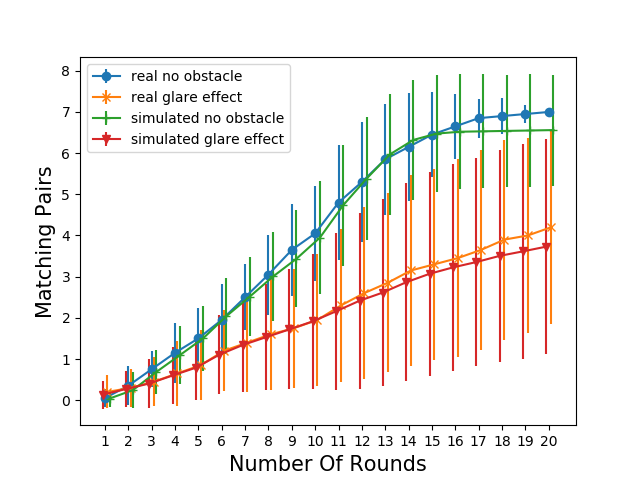
\includegraphics[width=8cm]{images/sd10x/Figure_3.png}
		\caption[Bild kurz]{Add caption}
		\label{fig:simOp101}
	\end{figure}
\end{minipage}
\begin{minipage}{0.5\textwidth}
	\begin{figure}[H]
		\centering
		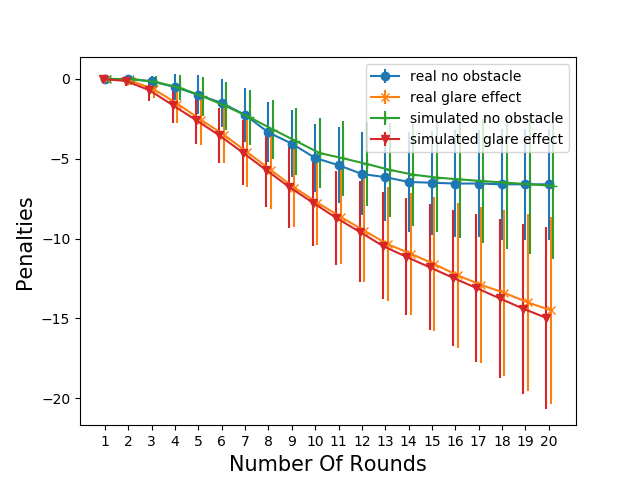
\includegraphics[width=8cm]{images/sd10x/Figure_4.png}
		\caption[Bild kurz]{Add caption}
		\label{fig:simOp102}
	\end{figure}
\end{minipage} 

Interestingly, including all the simulated data in the tests, results in less undesired result before the changes to the simulator compared to afterwards, but using only a small subset of the data results in the opposite. Before the changes to the simulator, when including only the best 10 games and the first 10 rounds in the tests, only one of the 4 tests comparing real and simulated games of the same mode show no significant difference. This is shown in table \todo{ref} and \todo{ref}. Contrary to that, after the changes to the simulator, the test on the chosen subset result in 3 out of those 4 tests show no significant difference. 

As all but one test produce desired results after the changes to the simulator, additional searches for a configuration that only shows desired resultrs were done.
However, such a configuration was not found. If less simulations are used, the three formerly significant differences become insignificant, but the difference in matching pairs bewtween simulated and real glare eeffect games becomes significant. Therefore using the 10 best simulations and the first 10 steps is a good compromise. It should be empghazised that this does not mean that the simulation of the glaree ffect games is bad reagrding the number of matching pairs per round. This only means that the paired sample t-test finds a significant difference in that comparisson. If the two lists of mean values that supposedly are significantly different are manually compared it can be seen that in reality the difference is very small. These values can be seen in table \todo{ref}.

\begin{table}[H]
	\centering
	\caption{mean values of matching pairs for real and simulated games. sd10x. for the first 10 rounds}%\label{tab1}
	\begin{tabular}{|c|c|c|c|c|c|c|c|c|c|c|}
		\hline
		& r1   &  r2  & r3 & r4   &  r5  & r6& r7   &  r8  & r9	&	r10\\
		\hline
		real&0.2 &0.3	&  0.45  &  0.65   &0.85 &  1.2   &    1.4 & 1.6 &  1.75 &1.95	\\
		\hline
		simulated&0.135 &0.27 &	0.405 &0.6  & 0.79 & 1.105& 1.34 & 1.53 & 1.72 & 1.915		\\
		\hline
	\end{tabular}
\end{table}

The highest mean differnece is in round 6 with a differnece of 0.095 matching pairs in that round. This shows that it does not mean that all glare effect simulations used are bad regarding the matching pairs, only because the statistical test finds a significant difference. 
%The fact that the paired sample t-test concludes a significant differnece could be related to the fact that the range of the value sis very small ranging only from .. to .. meaning a samall differnece is much according tpo the ttest..\todo{checken ob das logisch ist, also gucken was der ttest überhaupt macht und das begründen} (auschnitt beschrieben wenn ich weniger nehme.). This would also fit with the fact that using more steps and therefore having a bigger range of values for matching pairs in glare effect games, the difference is not significant (see example where all data is used, ref).

\subsection{Conclusion of the evaluation}
Although no configuration in which all simulations have no significant difference to the according real games regarding the paired sample t-test was found, it can be said that the simulator is capable to simulate the first 10 rounds very accurately, given only the 10 best simulations are used. The statistical tests and the previous consciderations regarding the too large standard deviation in later turns indicate, that the simulator performs less good in later turns. Having said that, these are only indications that would need further tuning and testing of the simulator to be confirmed. Doing so might lead to improving the simulator. 

Regarding the examination whether the changes to the simulator improved the overall quality of the simulations, no clear statement can be made. When all simualted data is used, the paired sample t-tests indicate, that the quality of the simulations may have gotten worse, while when using only the best 10 simulations and only the first 10 rounds, the tests indicate the opposite. 

This analysis also indicates, that it might not ideal to use all simulated data for training as that could results in a significant difference between the simulated and the real games. Using to many simulations compared to real games could decrease the performance of the classifeirs on real data if they adapt too much to simulated games. Furthermore is should be analysed how using differnet amounts of turns in the classification impacts the classification results. In section \todo{ref} different configurations regarding ratios of simulated to real games and the number of rounds includes, are tested. 

Nonetheless it should be emphasized that the aim of no significant difference between real and simuleted games is set very high. Overall the simulations and real games are very similar when comparing them with the two performance measurements. If only the best simulations are used the performance becomes even more similar.  

There are many options in choosing a subset of the data or adjusting the various parameters of the simulator, which could encance the quality of the simulations or reveal further aspects of the simulator that could be improved. In that sense, this analysis does not claim to be complete.

\begin{comment}
	Inhalt...
\end{comment}



\section{Feature generation}
\label{feature_generation}

\subsection{1D CNN features}
\label{1d_cnn_features}
For the 1D CNN five statistcal features for each step are used: The card codes, the number of cards left, the number of never revealed cards,  the highest number of times the same card was revealed and the number of steps  since all pairs were found. They are calculated using the game logs from \todo{ref}. These features can be direclty fed into the 1d CNN explained in chapter \todo{ref}. 

The code for calculating the statistal features out of game logs was already given. A script was written that incorparates this funtionality in order to calculate the features for all logs. Additionally, after creating the neccessary directory structure the script saves the files for the splits of the raw data and the features. The reason for saving the features is that they do not have to calculated before evrey training and instead can be loaded from files. The reason for also saving the raw data even though this work does not need them anymore is, that the working group that was collaborated with also trained other models and does not directly load the features but instead caalculates them before each training.

\subsection{2D CNN features}
\label{2d_cnn_features}

For the second approach of using a 2D CNN further steps are taken. Therefore synthetic images in gray scale colours are created using the features mentioned above. As the images are in gray scale colours, only one color channel is needed. One can visually think of this approach as creating graphs for each feature that display their values in each timestep, taking a photograph of each graph and stacking them on top of eachother. This can be clarified by looking at the code that produces the synthetic images.  

\begin{lstlisting}[language=python, caption=Add caption, xleftmargin=5.0ex]
def create_image(game, components=[True, True, True, True, True]):
	'''
	Creates synthetic images out of the five staticial features.
	:param game: The statical features in each step. 
	:param components: Five values describing which of the features 
	should be used to create the image. 
	:return: The synthetic image.
	'''
	card_codes = np.zeros((7, steps))
	cards_left = np.zeros((8, steps))
	never_revealed_cards = np.zeros((14, steps))
	max_same_card_reveals = np.zeros((20, steps))
	rounds_since_done = np.zeros((27, steps))
	
	x_position = 0
	for step in game:
		card_code = math.floor(step[0])
		first_or_second = int(round((step[0] % 1) * 10))
		if card_code != 0:
			card_codes[card_code - 1][x_position] = first_or_second 
		pairs_left[int(step[1] / 2)][x_position] = 1
		never_revealed_cards[int(step[2])][x_position] = 1
		max_same_card_reveals[int(step[3])][x_position] = 1
		rounds_since_done[int(step[4])][x_position] = 1
		x_position += 1
	
	image = np.zeros((0, steps))
	if components[0]:   
		image = np.vstack((image, card_codes))
	if components[1]:
		image = np.vstack((image, max_same_card_reveals))
	if components[2]:  
		image = np.vstack((image, rounds_since_done))
	if components[3]:
		image = np.vstack((image, cards_left))
	if components[4]:   
		image = np.vstack((image, never_revealed_cards))
	
	return image
\end{lstlisting}

By using pseudo colors, the images can be displayed with colours, like in figure \ref{fig:synImOr}. These 76 $\cdot$ 40 $\cdot$ 1 (height $\cdot$ width $\cdot$ colour channels) images are direclty fed to the 2D CNN explained in chapter .. \todo{rerf}. By setting the origin of the image to the lower instead of the upper left corner a more naural looking image is created and can be seen in figure \ref{fig:synIm}. 

\begin{minipage}{0.5\textwidth}
	\begin{figure}[H]
	\centering
	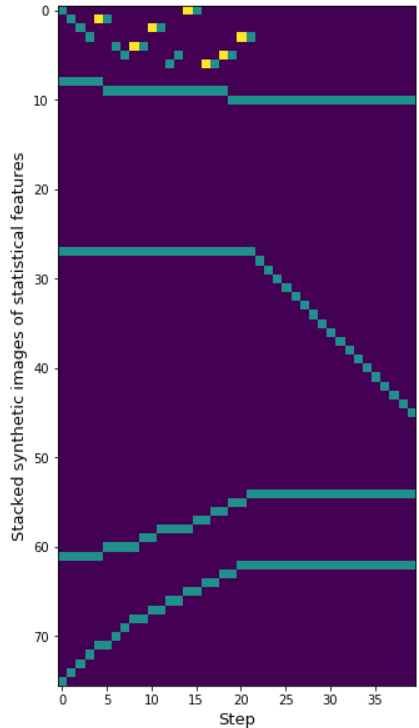
\includegraphics[width=7cm]{images/synImageOriginal.png}
	\caption[Bild kurz]{Add caption}
	\label{fig:synImOr}
\end{figure}
\end{minipage}
\begin{minipage}{0.5\textwidth}
	\begin{figure}[H]
		\centering
		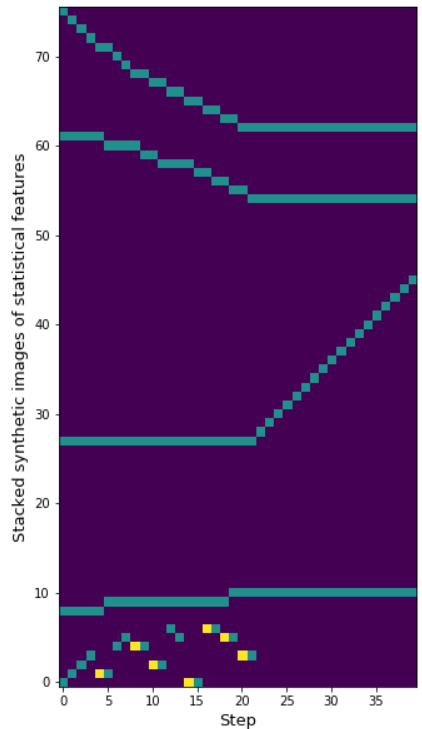
\includegraphics[width=7cm]{images/synImage.png}
		\caption[Bild kurz]{Add caption}
		\label{fig:synIm}
	\end{figure}
\end{minipage}

The width of the image is 40 because that the number of steps recorded. Table \todo{ref} shows which of the areas in the image describe which statical feature. The different vertical spaces given to statistical features were purposefully chosen. The aim was to use as much space as neccessary but as little as possible. As each round consists of two cards being turned face up and the impossibility to chose the same card twice in one turn, a card can be at maximum revealed 20 times during 20 rounds. Considering that this value is at minimum 1 because it is not possible to flip no cards, the range of 20 values is sufficient for this value. Furthermore 14 steps are at minimum needed to complete the game, since there are 14 cards. As a result this value can range from 0 to 26, meaning a vertical space of 27 is needed. In order to save space, the statistcal feature of the number of cards left was converted to the number of pairs left. By dividing by 2 the vertical space neccessary to visualize this feature is halved, without information being lost. Instead of representing the numbers left on the field, the value now represents the number of pairs left. Furthermore the number of never revealed cards can range from 0 to 13. The value 14 is not possible because two cards have to be chosen each turn, meaning that it is impossible to not reveal any card. The stacking order was chosen so that the coloured pixels of different statistical features rarely touch each other. 
\begin{table}[H]
	\centering
	\caption{add caption. Upper and lower boundaries are inclusive.}%\label{tab1}
	\begin{tabular}{|l|l|l|}
		\hline
		Statistical feature & Range & Vertical space in the image \\
		\hline
		Card codes & 1-7 & 0-6 \\
		Maximum of same card reveals & 1-20 & 7-26 \\
		Steps since game ended & 0-26 & 27-53 \\
		Pairs left & 0-7 & 54-61\\
		Never revealed cards & 0-13 & 62-75 \\
		\hline
	\end{tabular}
\end{table}

Regarding the visual representatoin of he card codes two two decisions were made: Using different colours for the first and the second card of a colour and combining the information about the 14 cards in an vertical area of size 7. For each card code the vertical position of the representing pixel is decided by the first number and the colour is chosen according to the second number. As a result each row contains the information about cards of a specific colour. This representation of the card codes is not chosen arbirtrarily. On the contrary, it was inspired by reasons that need explanation.

Insrtead of combining the information about the 14 cards in an vertical area of size 7, it would have been also possible to use double the vertical space so that the first and the second card of a colour each have separate areas. The first cards and the second cards of a colour would each have individual vertical spaces with sizes of 7. However, it was decided against it. This decision was based on a conscideration regarding the way convolutional neural networks function and how they are used in this work. How cnns function is discussed in detail in chapter \todo{ref} and therefore the following explanation is kept short. During a convolution, each filter has a fixed size and step by step walks over the image, extracting features from areas to create a feature map. This means that a neuron in this layer only reacts to stimuli in a local area of the previous layer. \todo{satz selsbt verstehen und gucken ob ich es umschreieb dass es verständlicher ist. auf jeden fall auch in cnn chapter aufgreifen} This behaviour follows the biological model of the receptive field. As cnns consist of multiple layers, the receptive field, and therefore the distance in which dependencies between the pixels in the original input image can be learned, grows with each layer. This also means that if the structure of the cnn is chosen small, its receptive field might not grow enough for the model to learn dependencies between far distant pixels of the original input image. In this work, the 2d cnn used is intentionally constructed with a small number of layers for reasons explained in chapter \todo{ref}. Therefore it is desireable that pixels in between an important dependency can be assumed are close to each other so that the small cnn is able to learn that dependency. %Firstly, more complex structures were tested on the synthetic images and did not show better results, meaning that small networks are sufficient for the task at hand and secondly, less complex models result in shorter training time and by that allow the training of more models. 
Unlike in classical image classification the images used are created synthetically, and in that sense their structure can be chosen freely in the favour of the task at hand. The chosen representation of the card codes exploits exactly this freedom. As the dependencies between cards of the same colours can be estimated to be very important for the classification, the representation is chosen so that if cards of the same colour are flipped in quick succession the pixels describing them are also locally close to each other in the synthetic image. The dependency between such close pixels does not require a large receptive field in order to be learned by the network. Therefore this representation is better suited for the small structure of the cnn that is being utilized. 




%a representation is chosen in which pixels describing cards of the same colour are in the same row and have different colours depending on if it is the first or second card of that colour. As a result, . Additionally these visual  properties are less complex than they would have been in the other approach and are therefore more 

%when conscidering how convoluntions in 2d cnns are performed, this approach seems less promissing. During the convolutions, each filter has a fixed size and step by step walks over the image, extracting features from areas to create a feature map \todo{ref to cnn chapter}. This means that the extracted features during a convolution and therefore the gained knowledge of the model depends on the information found in areas with the size of the filter. Regarding the topic at hand, chossing individual areas for the card codes would create a significant distance between the pixels describing the first and second card of a colour. In order to extract features during the convolution that capture the connection between those distaned pixels, the filter size would need to be at least as big as the distance. This results in large areas that include many different pixels overshadowing the importance of the two specific pixels  describing the first and the second card of a color and thereby making it harder for the model to learn the connection between them. Hence, the approach of doubling the vertical space results in high unlikelyness of the model learning this characteristic. Contrary to that, using a combined space and different colours results in spatial proximity of the pixels describing the desired characteristic, which can therefore be captured by smaller filter sizes. In conlusion, chossing a representation for the card codes that contains local features and using a small filter size, results in a higher likelyness of capturing the desired characteristics. 

The main reason that motivated the use of different colours derived from the first decision to combine information about 14 cards in a vertical space of 7. If the same colour was used for all card codes, there would be no visual differnece between flipping the same card in consequtive turns and flipping two different cards with the same colour. This of course would also mean that the model could not differentiate bewteen those two cases, although they stem from completely differnet behaviour. Using different colours for the first and the second card of a colour fixes this issue. Furthermore the colours visually emphasize some behavioural characteristics that could be helpful for the eventual classifier. By comparing the the card code sections of two images from which one is created using a glare effect and the other one with a no obstacle game, using different colours results in noticeably different visual representations. 
\begin{figure}[H]
	\centering
	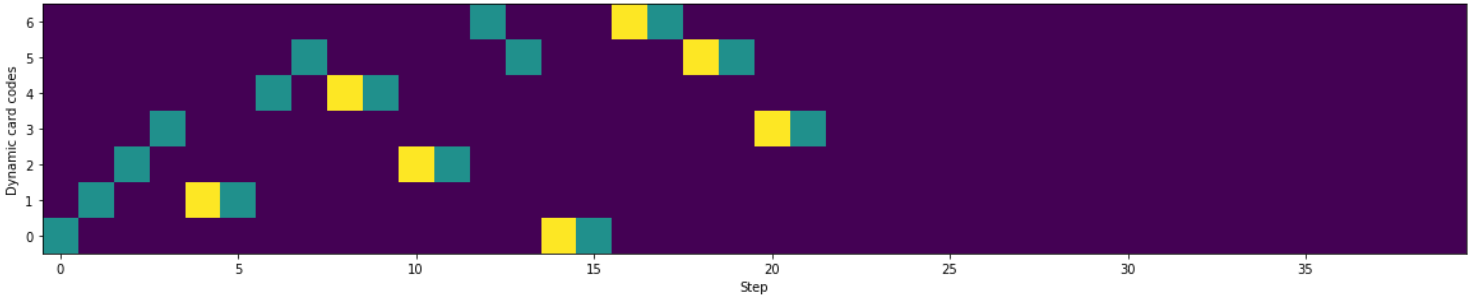
\includegraphics[width=15cm]{images/cardCodesNoObst.png}
	\caption[Bild kurz]{Add caption}
	\label{fig:ccNo}
\end{figure}
\begin{figure}[H]
	\centering
	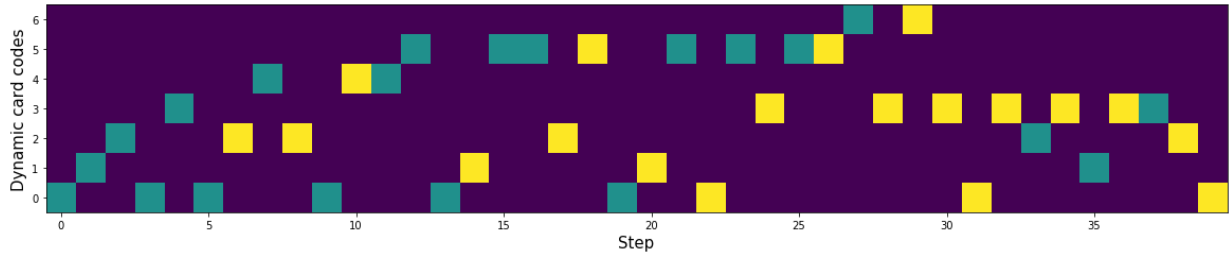
\includegraphics[width=15cm]{images/cardCodesGlare.png}
	\caption[Bild kurz]{Add caption}
	\label{fig:ccGlare}
\end{figure}
In \ref{fig:ccNo}, showing the image for an no obstacle game, there are yellow pixels directly left of green ones, meaning that the probant flipped a card, knew that he had already seen the matching card and direclty flipped it. However, this happens less often in figure \ref{fig:ccGlare} which shows the image for an glare effect game. This is not the case in every game, but the theory is that separations of different coloured cells in the image are more likely in glare effect games than in no obstacel games. Therefore it could be beneficial for the model to learn these characteristics. It should be noted that what the cnn exactly learns or what exact influence the chosen representation has can only be speculated. 

%It could be argued that simply using a vertical space of 14 and changing the order of the rows so that rows describing cards of the same colours are next to each other would have been an easier solution. However, this would firstly be contradicting to the aim using as little space as neccessary and secondly would exclude the possibility of emphasized behavioural characteristics that 

Especially the uncertainty in the influence of the different colours shows, that the approach of creating synthetic images is very experimental. There is no such thing as a standard approach in creating synthetic images for cnns. At least there is none, yet. Although the way cnns function can be conscidered when deciding how to create the synthetic image, this does not guarantee good classification results.


\begin{comment}
	The idea behind using different colours for the first and the second card of a colour is that this vizualizes important behavioural characteristics that help deciding whether the visual obstacle being the sunlight is involved or not. By comparing the the card code sections of two images from which one is created using a glare effect and the other one with a no obstacle game, the different colours result in a noticeably . 
	\begin{figure}[H]
	\centering
	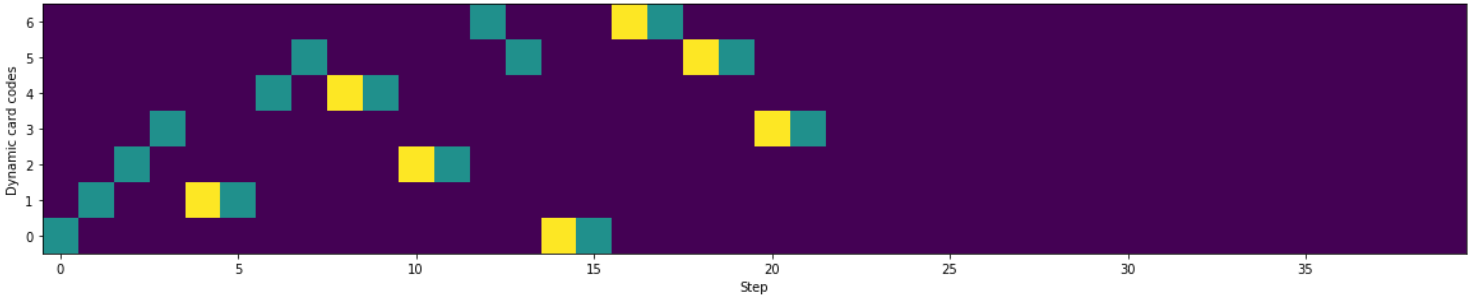
\includegraphics[width=15cm]{images/cardCodesNoObst.png}
	\caption[Bild kurz]{Add caption}
	\label{fig:ccNo}
	\end{figure}
	\begin{figure}[H]
	\centering
	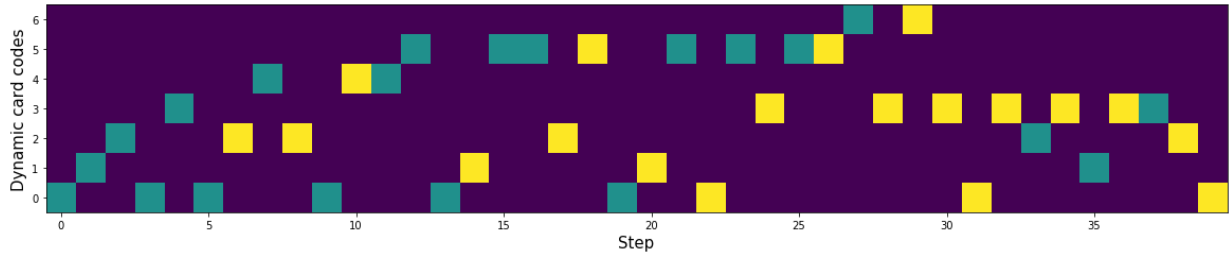
\includegraphics[width=15cm]{images/cardCodesGlare.png}
	\caption[Bild kurz]{Add caption}
	\label{fig:ccGlare}
	\end{figure}
	
	In \ref{fig:ccNo}, showing the image for an no obstacle game, there are yellow pixels directly left of green ones, meaning that the probant flipped a card, knew that he had already seen the matching card and direclty flipped it. However, this happens less often in figure \ref{fig:ccGlare} which shows the image for an glare effect game. This is not the case in every game, but the theory is that separations of different coloured cells in the image are more likely in glare effect games than in no obstacel games. Therefore it could be beneficial for the model to also learn these characteristics. If the same colour was used for all card codes, there would be no visual differnece between flipping the same card in consequtive turns and flipping two different cards with the same colour. This of course would also mean that the model could not differentiate bewteen those two cases.
	
	It 
\end{comment}

umschrieben: grund ist, dass es zusätzliche characteristekn des spiels visualisiert, die von den convolutional genauer gesgat dem rezepivem feld erfasst werden können. ... zeigen und erklären .. bei 14 reihen und getrennt jeweils für erste ode zweite wären die pixel die gefundene paare beschrieben nicht in der nähe voneonader. Ein kleines rezeptive feld würde könnte den zusammenhanmg nicht erfassen. Und selbst wenn man ein größeres wählt gibt es in dem bereich des feldes dann deutlich mehr pixel mit dem selben farben die den wichtigen zusammenhang zwischen 2 spezifischen pixeln in den schatten stellen könnten. Würde man gleiche farben benutzen gäbe es keinen untershcied zwischen zweimal die selbe karte in nah einanderfolgenden zügen und die zueinandergehörigen beiden karetn. Es heißt jedoch nicht dass das netz nicht in der lage ist featurees (oder so) aus verschiedenen bereichen in verbindung zu setzen. Ganz im gegenteil: die fullyy connected oder auch dense layer tun genau dies. Jedoch suchen sich die fully connected layer quasi die feautures aus dem letzen vorherigen layer aus die wichtig sind. Aber angenommen die beiden angesprochen pixel sind sich nicht nah genug um vom rezeptiven field erfasst zu werden und zwischen den beiden pixeln bzw. generell in dem bereich der card codes sind noch viele weitere solcher pixel, dann gibt es keine features die den zusammenhang enthalten und die aufgabe diesem ztusammenhang zu finden liegt dann an den dense layern. Das die dense layer einen zusammenhang zwischen genau den beiden pixln finden und das für gänzlich unterschiedliche card code bereiche je spiel ist äußerst undwahrscheinlciu. \todo{das muss biscchen genauer und verständlicher alles.}

\todo{text}

\todo{vielleicht mit mazen drüber reden ob das sinn ergibt. Ich glaube das ergibt sinn, aber ich müsste nochmal mehr das quellen suchen. Auch mir receptive field und so}
